%\documentclass[11pt]{article}
\documentclass[journal,onecolumn,11pt]{IEEEtran}

\usepackage{blindtext}
\usepackage{etoolbox}
\usepackage{graphicx}

\makeatletter
\def\do#1{\patchcmd{#1}{\thepage}{\null}{}{\GenericWarning{}{Could not patch \string#1}}}
\docsvlist{\@oddhead,\@evenhead,\ps@headings,\ps@IEEEtitlepagestyle,\ps@IEEEpeerreviewcoverpagestyle}
\makeatother

\usepackage{cite}
\usepackage[T1]{fontenc}
\usepackage[utf8]{inputenc}
\usepackage[left=1in,right=1in,top=1in,bottom=0.8in]{geometry}
\usepackage[bookmarks=false,pdfstartview=FitH,colorlinks,citecolor=blue,filecolor=green,linkcolor=blue,urlcolor=blue]{hyperref}
%\usepackage{bookmark}
%\usepackage[bookmarks=false,pdfstartview=FitH,bookmarksopen=true]{hyperref}
\usepackage{url}
\usepackage[caption=false,font=footnotesize]{subfig}
%\usepackage{fixltx2e}
\usepackage{stfloats}
% this is the preamble
% put all of the above code in here
%\usepackage{setspace}
\setlength{\parskip}{0.5em}

%\makeatletter% since there's an at-sign (@) in the command name
%\renewcommand{\@maketitle}{%
%  \begin{center}
%    \parskip\baselineskip% skip a line between paragraphs in the title block
%    \parindent=0pt% don't indent paragraphs in the title block
%    {\bf\@title}\par
%    \textbf{\@author}\par
%    \@date% remove the percent sign at the beginning of this line if you want the date printed
%  \end{center}
%}
%\makeatother% resets the meaning of the at-sign (@)

\title{Report on Data Centers}
\author{\IEEEauthorblockN{Yongsen MA}
%\IEEEauthorblockA{mayongsen@gmail.com, http://yongsen.github.com}
}
%\markboth{I\MakeLowercase{nterview for} P\MakeLowercase{h}D A\MakeLowercase{pplication of} CS,HKU}{Yongsen MA}

\begin{document}

\maketitle% prints the title block
%\onehalfspacing

\section{Literature Review}

According to the architecture and topology in these papers, Data Center Networks can be divided into:
\begin{enumerate}
  \item Static-electrical:
  \begin{enumerate}
    \item Multi-layer tree:
        \begin{enumerate}
          \item Fat-tree \cite{Al-Fares:2008:SCD:1402958.1402967}
          \item VL2 \cite{Greenberg:2009:VSF:1592568.1592576}
        \end{enumerate}
    \item Server-centric:
        \begin{enumerate}
          \item DCell \cite{Guo:2008:DSF:1402958.1402968}
          \item BCube \cite{Guo:2009:BHP:1592568.1592577}
        \end{enumerate}
    \item Random graph:
        \begin{enumerate}
        \item Jellyfish \cite{singla2012jellyfish}
        \end{enumerate}
    \item Multi-tenant:
        \begin{enumerate}
        \item NetLord \cite{Mudigonda:2011:NSM:2018436.2018444}
        \item Oktopus \cite{Ballani:2011:TPD:2018436.2018465}
        \item FairCloud \cite{Popa:2011:FSN:2070562.2070584}
        \end{enumerate}
  \end{enumerate}
  \item Flexible:
  \begin{enumerate}
    \item Optical:
    \begin{enumerate}
      \item c-Through \cite{Wang:2010:CPO:1851182.1851222}
      \item Helios \cite{Farrington:2010:HHE:1851182.1851223}
      \item OSA \cite{chen2012osa}
    \end{enumerate}
    \item Wireless:
    \begin{enumerate}
      \item Wireless flyways \cite{Halperin:2011:ADC:2018436.2018442}
      \item 3D beamforming \cite{Zhou:2012:MMC:2342356.2342440}
      \item Cylindrical racks \cite{Shin:2012:FCW:2396556.2396560}
    \end{enumerate}
  \end{enumerate}
\end{enumerate}

These papers mainly discussed the issues of:
\begin{itemize}
  \item Topology \cite{Al-Fares:2008:SCD:1402958.1402967,Greenberg:2009:VSF:1592568.1592576,Guo:2008:DSF:1402958.1402968,Guo:2009:BHP:1592568.1592577,singla2012jellyfish}
  \item Addressing \cite{Al-Fares:2008:SCD:1402958.1402967,Greenberg:2009:VSF:1592568.1592576}
  \item Mapping \cite{Chen:2010:GAA:1851182.1851190,Greenberg:2009:VSF:1592568.1592576}
  \item Routing \cite{Guo:2008:DSF:1402958.1402968,Guo:2009:BHP:1592568.1592577}
  \item Scheduling \cite{Al-Fares:2008:SCD:1402958.1402967,Halperin:2011:ADC:2018436.2018442}
  \item Failure handling \cite{Chen:2010:GAA:1851182.1851190,NiranjanMysore:2009:PSF:1592568.1592575,Wu:2012:NAD:2342356.2342438}
\end{itemize}

\subsection{Static-electrical Data Centers}

The traditional data centers are generally designed in static connection by electrical switches. For the issues of topology, routing and scheduling in these data centers, there are numerous researches in this field including Fat-tree \cite{Al-Fares:2008:SCD:1402958.1402967}, VL2 \cite{Greenberg:2009:VSF:1592568.1592576}, DCell \cite{Guo:2008:DSF:1402958.1402968}, BCube \cite{Guo:2009:BHP:1592568.1592577}, Jellyfish \cite{singla2012jellyfish}, etc. These work can be classified into multi-layer tree, server-centric and random graph according to the differences in topology graph, which also brings different advantages and disadvantages.

\subsubsection{Multi-layer Tree}

The topology of fat-tree is multi-rooted tree which can provide full aggregate bandwidth with low cost and resolved the bottleneck in inter-node communication. But the scale of fat-tree is limited that $48$-port switches can only support $48 \cdot \frac{48}{2} \cdot \frac{48}{2}=27648$ hosts at most.

The conventional data center architecture has limited server-to-server capacity that the over-subscription ratio increases rapidly in upper layer switches. Also, servers in multi-layer tree are location related that nearby servers are responsible for demand peaks or failures resulting in resources wasting. According to the measurement and analysis of traffic patterns, VL2 adopts Virtual Layer 2 Networking to realize the dynamic resource allocation across large server pools. It can assign any server to any service which can address the fluctuating demands of individual services.

The multi-rooted tree topology has poor fault-tolerant features which make it hard to detect and maintain failures. Furthermore, multi-rooted tree can not support one-to-all and all-to-all communications effectively.

%Addressing: Pod: 10.pod.switch.1, core: 10.k.j.i, host: 10.pod.switch.ID

\subsubsection{Server-centric}

For server-centric data centers, all-to-all communication can be realized and the network can be incrementally expanded. DCell is a recursively defined structure which scales doubly exponentially as the node degree increases (ideal for large scale data centers). Furthermore, DCell is fault tolerant and can provide higher network capacity. But the bottleneck link locates in the low-level links and traffics are not balanced. Moreover, increment expansion requires additional ports which brings extra overhead and complexity.

%Topology:
%$n$ servers connected to a mini-switch within $DCell_0$, then $DCell_k$ is recursively generated by $t_{k-1}+1$ $DCell_{k-1}$s. The number of servers scales doubly exponentially as the node degree increases.
%
%Addressing:
%a server in $DCell_k$ is denoted by $[a_k,uid_{k-1}]$, where $a_k$ is the $DCell_k$ this server belongs to and $uid_{k-1}$ is the unique ID of the server inside this $DCell_{k-1}$.
%
%Routing: find the connection $(n_1,n_2)$ between $DCell$s, then find the paths of $src$ to $n_1$ and $n_2$ to $dst$. When failures occur, choosing \textit{proxy} to make local-reroute or jump-up (rack failure).

BCube provides a similar server-centric solution for modular data centers, which has no performance bottlenecks and provides much higher network capacity. However, to connect certain number of servers, it needs more switches ($k$ times) and wiring is more complex which will increase the cabling cost. For BCube, the aggregate bottleneck throughput decreases gracefully under both server and switch failures, which means poor performance when incomplete units exit.

In the multi-path routing and speedup forwarding of one-to-all communications, it needs \textbf{strict time synchronization}, and more importantly, brings the trade-off of reliability and capacity just as MIMO in wireless networks.

%Topology:
%$BCube_0$ is $n$ servers connecting to an $n$-port switch. $BCube_k$ is constructed from $n$ $BCube_{k-1}$s and $n^k$ $n$-port switches.
%
%Addressing:
%servers: $a_ka_{k-1}\cdot\cdot\cdot a_0$ ($a_i\in [0,n-1],i\in [0,k]$); switches: $<l,s_{k-1},s_{k-2}\cdot\cdot\cdot s_0>$, where $l$($0\leq l\leq k$) is the level of the switch.
%
%Routing:

\subsubsection{Random Graph}

The architectures listed above have rigid structure that interferes with incremental expansion. Jellyfish adopts random graph topology to address this problem, and also provides great flexibility in oversubscription design. But it brings challenging complexity to routing, wiring and maintaining.

\subsection{Flexible Data Centers}

\subsubsection{Optical}

\textbf{"OSA: An Optical Switching Architecture for Data Center Networks with Unprecedented Flexibility", NSDI 2012}

\textbf{"c-Through: Part-time Optics in Data Centers", SIGCOMM 2010}

\begin{enumerate}
  \item optical circuit switching: high bandwidth but large delay (low bisection bandwidth)
  \item convert routing to multiplex
  \item separating the networks of packet-switch and circuit-switch increases the configuration complexity
  \item buffer adds overhead
  \item buffer at end hosts but not switches: requires hosts be programmable
  \item weighted perfect matching problem: take traffic loads and capacity into consideration
  \item each host runs a management daemon: adds overhead
  \item artificially use an Ethernet switch to emulate the optical switch: accuracy
\end{enumerate}

\textbf{"Helios: A Hybrid Electrical/Optical Switch Architecture for Modular Data Centers", SIGCOMM 2010}

the available bisection bandwidth is inflexible for predefined topology

\begin{enumerate}
  \item unlike c-Through, Helios requires no modifications to end hosts but only at switches
  \item without debouncing and EDC will improve throughput, but will reduce goodput due to link insertion and signal noise?
  \item unidirectional circuits can better adapt to asymmetric traffic demands
\end{enumerate}

\subsubsection{Wireless}

\textbf{"Mirror Mirror on the Ceiling: Flexible Wireless Links for Data Centers", SIGCOMM 2012}

Wireless Data Center is a new concept which should be explored further. Many issues such as interference, secluding, security, etc. should be standardized. On the other hand, the issues on cost, performance, energy-efficiency, reliability, etc. should be taken into consideration compared with electrical or optical data centers.

%\begin{figure}[!t]
%\centering
%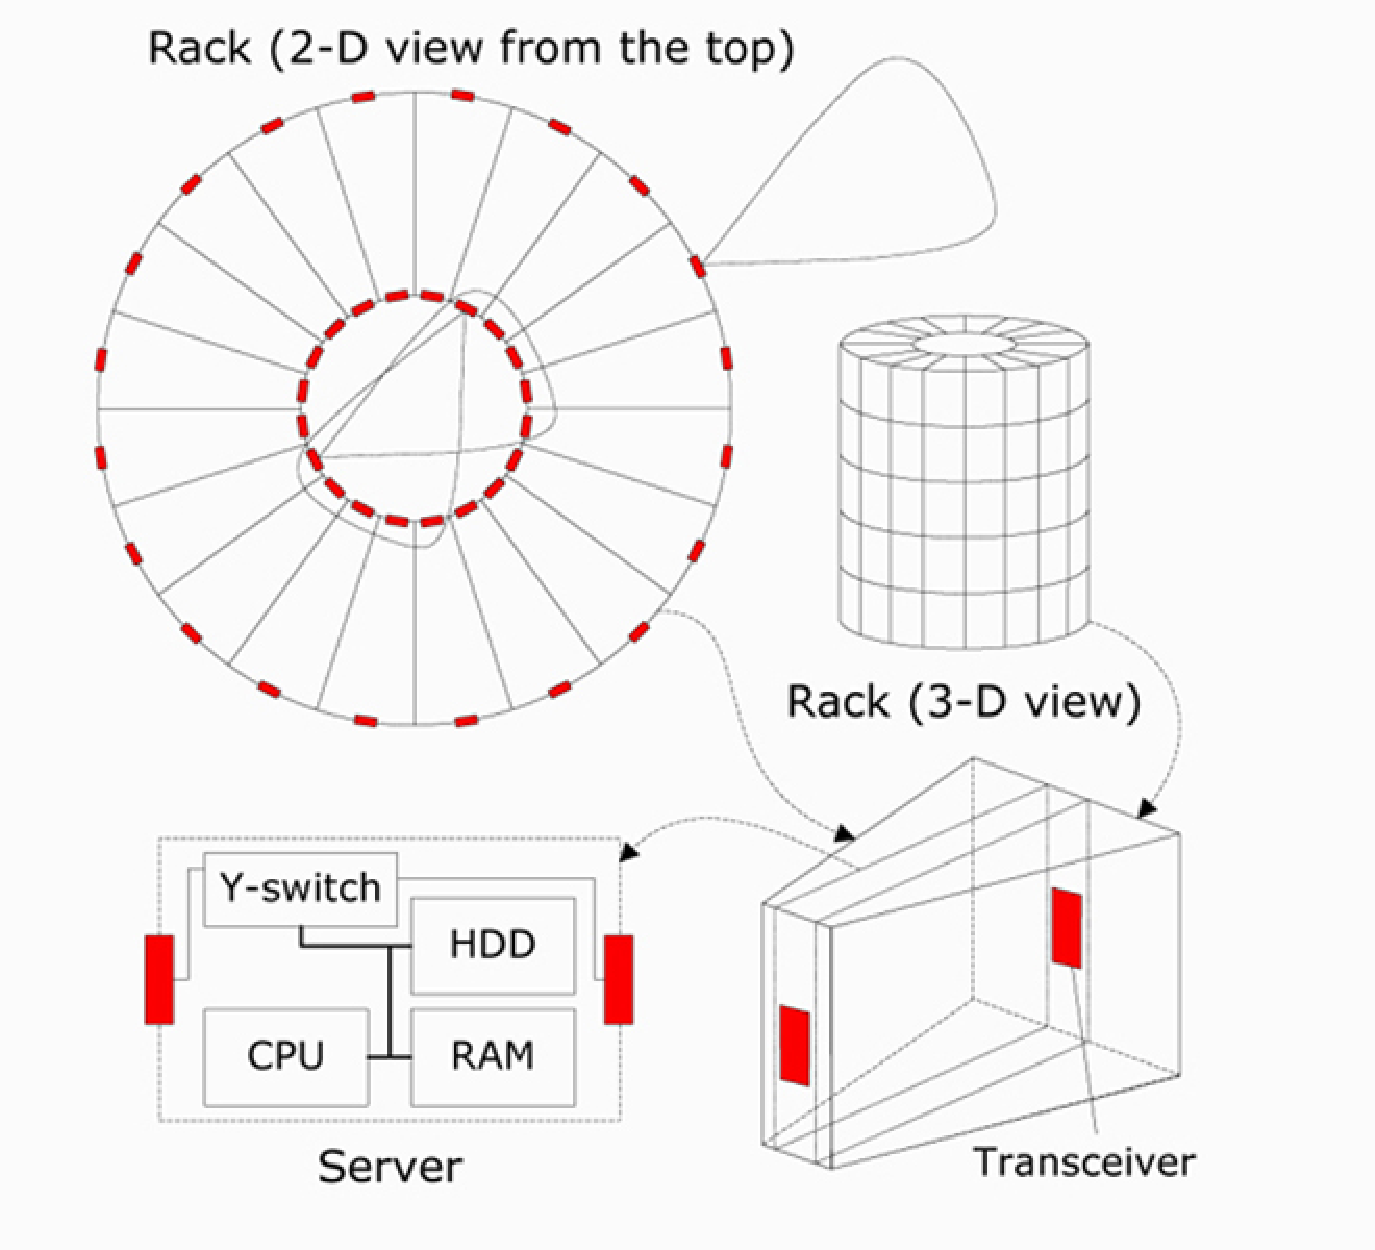
\includegraphics[width=0.4\textwidth]{wirelessdata.pdf}
%\caption{Possible solution: cylindrical racks}
%\label{cylindrical}
%\end{figure}

\begin{enumerate}
  \item electrical
  \item optical
  \item wireless
  \begin{enumerate}
    \item Link Blockage
    \item Radio Interference
  \end{enumerate}
\end{enumerate}

Max concurrent links: Link conflicts (SINR); Greedy scheduling (graph coloring); Assigning radios.

Problems:
\begin{itemize}
  \item Apart from the concurrent links, the efficient throughput should be explored. For instance, although the concurrent links are more with larger ceiling height $h$, it can decrease the throughput according to the curves of RSS (or Data Rate) vs. distance as shown in Figure 5.
\end{itemize}

\textbf{"Augmenting Data Center Networks with Multi-gigabit Wireless Links", SIGCOMM 2011}

"The base wired network is provisioned for the \textbf{average case} and can be oversubscribed. Each ToR switch is equipped withe one or more 60GHz wireless devices." "A central controller monitors DC \textbf{traffic patterns}, and switches the beams of the wireless devices to set up flyways between ToR switches that provide \textbf{added bandwidth} as needed." So it is ideal for \textbf{flexible and energy-efficient} data centers.

Problems:
\begin{itemize}
  \item Conflict graph: for $N$ racks and $K$ antenna orientations, the input table is very \textbf{large} with the size of $(NK)^2$. On the other hand, the propagation conditions are similar, i.e., the table is \textbf{sparse}.
\end{itemize}

\subsection{Other issues}

\subsubsection{Multi-tenant}

\textbf{"FairCloud: Sharing The Network In Cloud Computing", SIGCOMM 2012}

\textbf{"Towards Predictable Datacenter Networks", SIGCOMM 2011}

\textbf{"NetLord: A Scalable Multi-tenant Network Architecture for Virtualized Datacenters", SIGCOMM 2011}

\subsubsection{Failure Handling}

\textbf{"Generic and Automatic Address Configuration for Data Center Networks", SIGCOMM 2010}

Basic Procedures:
\begin{enumerate}
  \item O2 Mapping
  \begin{enumerate}
    \item Candidate selection via SPLD: \textbf{select} candidate with the same SPLD.
    \item Candidate filtering via orbit: \textbf{skip} candidate with the same orbit, then $Decomposition()$.
    \item Selective splitting $Refinement^*()$: \textbf{split} cells that really connect to the including cell.
  \end{enumerate}
  \item Malfunction Detection
  \begin{enumerate}
    \item Anchor pair selection:
    \item Malfunction detection:
  \end{enumerate}
\end{enumerate}

Problems:
\begin{enumerate}
  \item Initial selection of vertex $\nu\in\pi_p^i$
  \item Whether it can be resolved by Compress Sensing?
  \begin{enumerate}
    \item the topology graphs are sparse.
    \item only certain parts are changing in real-time operating (considering certain servers can be turned down for energy-efficiency and demand response).
  \end{enumerate}
\end{enumerate}

\textbf{"NetPilot: Automating Datacenter Network Failure Mitigation", SIGCOMM 2012}

\textbf{"PortLand: A Scalable Fault-tolerant Layer 2 Data Center Network Fabric", SIGCOMM 2009}

\section{Research Issues}

\subsection{Topology Control}

\begin{enumerate}
  \item topology graph is large and sparse
  \item topology graph is changing due to errors, multiplexing and demand response
  \item capacity differences in up- and down-link (directional graph)
  \item capacity differences in connections (weighted graph)
\end{enumerate}

Compress Sensing

\subsection{Demand Response}

according to the traffic measurement and analysis in VL2 and wireless flyways, traffic patterns and loads are dynamic and unpredictable. So demand response can be done by Lyapunov optimization for it only needs the information of current and previous state.

\subsection{Capacity Scheduling}

\subsection{Resource Allocation}

high efficiency: good trade-off between reliability and capacity

\section{Motivation}

With the increasing demand of traffic loads and user requirements, it is a great challenge to make data centers agile and energy-efficient. A basic solution is to allow dynamic resource allocation based on flexible data center networks. The recent development of 60GHz wireless technology opens a door for the deployment of flexible data centers. It provides a good choice of adding capacity to data centers with under-provisioning capacity design. However, this will lead to new problems such as topology control and capacity scheduling, apart from the wireless propagation and link adaption in wireless networks. The PHY and MAC standardization of 60GHz networks is still ongoing (WirelessHD and IEEE 802.11ad/WiGig), its application in data centers should be further explored for the specific feature of topology and services.

\begin{figure}[!htp]
\centerline{
    \subfloat[Provisioning for peak load]{
    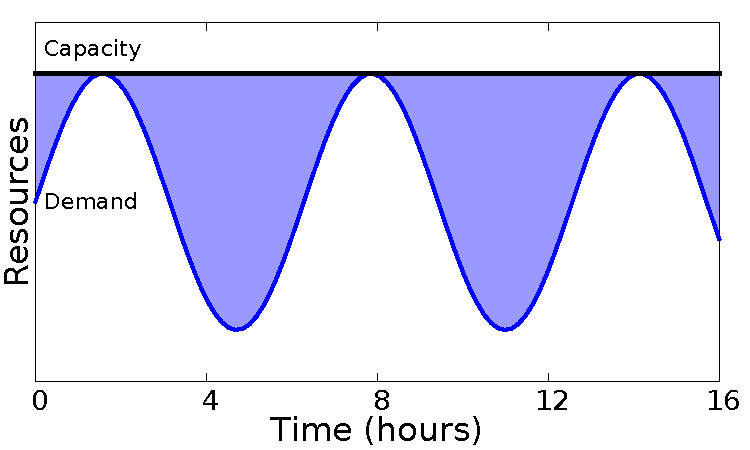
\includegraphics[width=0.33\textwidth]{capacity.pdf}
    \label{peak}
    }
    \subfloat[Fixed underprovisioning]{
    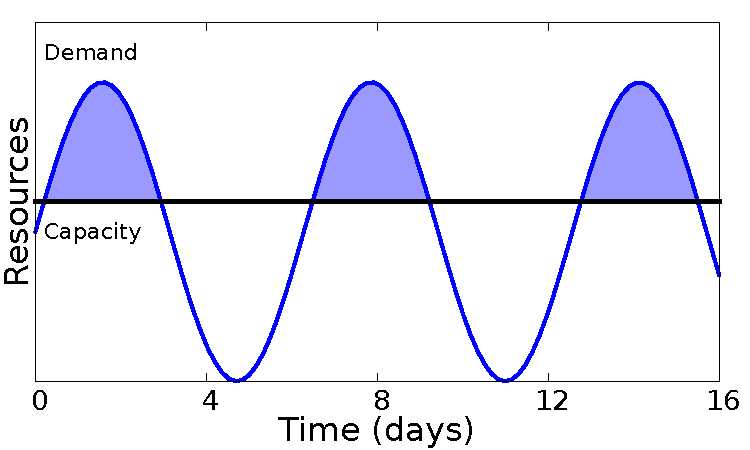
\includegraphics[width=0.33\textwidth]{capacity1.pdf}
    \label{under}
    }
    \subfloat[Flexible underprovisioning]{
    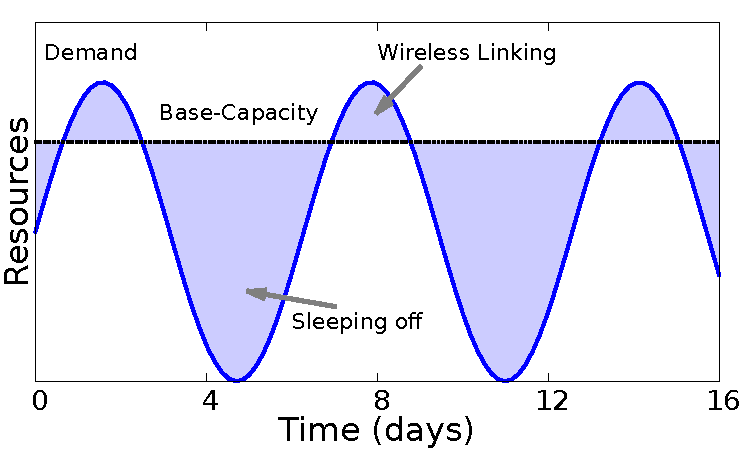
\includegraphics[width=0.33\textwidth]{capacity2.pdf}
    \label{under_wireless}
    }
}
\caption{Capacity provisioning based on traffic loads}
\label{provisioning}
\end{figure}

Generally, the capacity of data centers is designed for peak loads, as shown in Figure \ref{peak}, but the resources will be wasted during non-peak times \cite{Armbrust:2010:VCC:1721654.1721672}. On the other hand, if the capacity is designed in under-provisioning case as shown in Figure \ref{under}, the peak requirements can not be satisfied, leading to potential revenue sacrifice or over-occupied errors. To address these problems, we can employ flexible capacity and dynamic demand response, i.e., 60GHz wireless linking to add capacity for peak loads and sleeping mechanism to improve performance/cost efficiency, as shown in Figure \ref{under_wireless}.

The wireless-flexible data centers are generally composed of:
\begin{enumerate}
  \item Topology and Addressing:
  \begin{enumerate}
    \item Conflict Graph: Propagation table (wireless), capacity matrix (wired/wireless) and traffic loads table (wired/wireless)
    \item Topology Graph: Physical-specific ID Addresses (PAs), Logical-specific IP Addresses (LAs) and Application-specific IP Addresses (AAs)
        \begin{enumerate}
        \item PAs: providing distance information for 3D Beamforming
        \item LAs: providing topology information for Capacity Adaption
        \item AAs: providing traffic information for Demand Response
        \end{enumerate}
  \end{enumerate}
  \item Routing and Scheduling:
  \begin{enumerate}
    \item 3D Beamforming: adding additional capacity to neighbor ToRs according to PAs
    \item Demand Response: traffic estimation according to AAs
    \item Capacity Adaption: capacity scheduling according to LAs
  \end{enumerate}
\end{enumerate}

\section{Methodology}

The problems of topology control, addressing, routing, and scheduling also exit in traditional data centers, but it brings new challenges when wireless links are introduced. For instance, the topology graph is changing due to wireless links and on-demand response. Also, the capacity matrix and conflict graph of wireless links are closely related to the relative locations of servers, e.g., capacity of 6G for neighbor servers and 1/2G for non-neighbor servers. Furthermore, the measurement and mapping of topology graph, conflict graph and traffic loads is challenging for large scale data centers.

\begin{figure}[!htp]
\centering
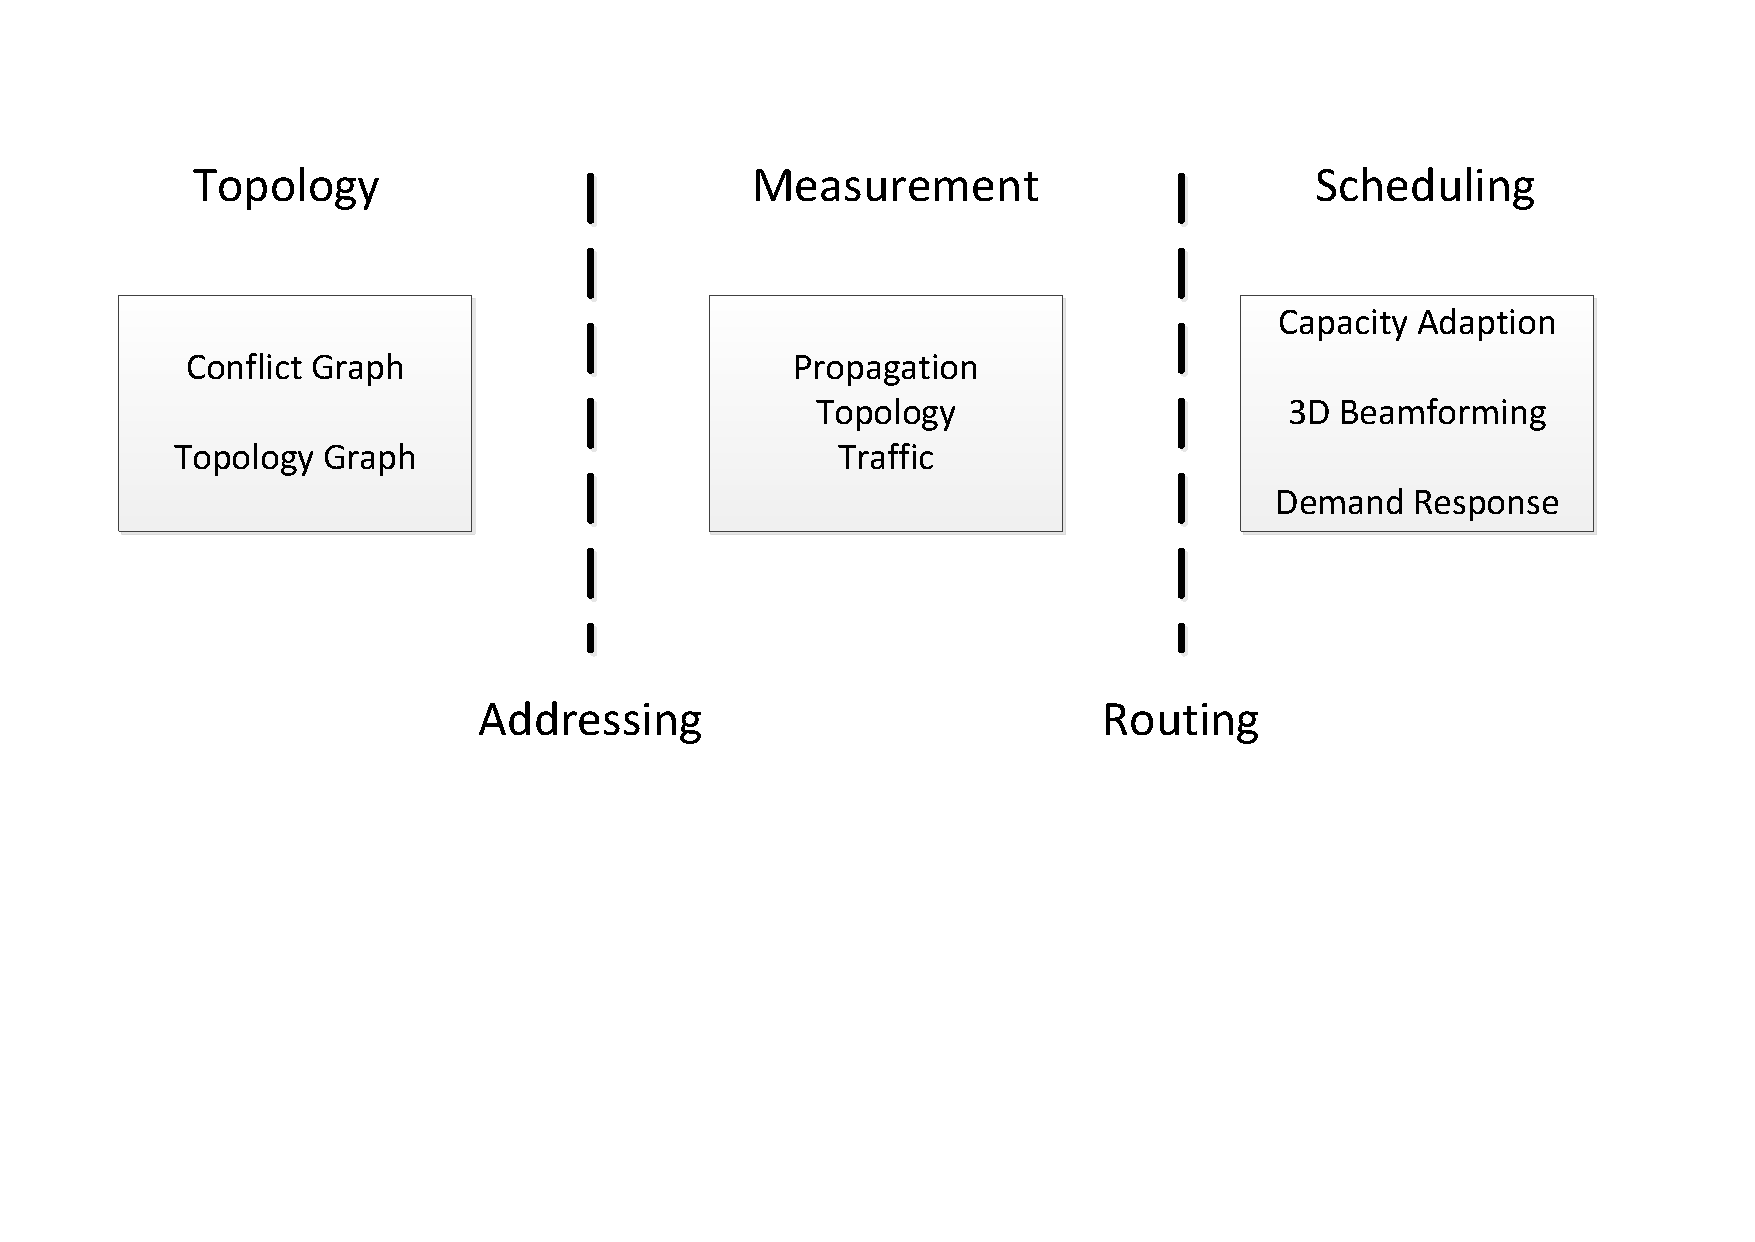
\includegraphics[width=0.8\textwidth]{framework.pdf}
\caption{Framework of flexible data centers based on 60GHz wireless networks}
\label{framework}
\end{figure}

Considering the scale of topology (conflict/topology graph and different addresses) and multi-layer scheduling (physical topology, capacity matrix and traffic patterns), we can employ \textbf{Compress Sensing} and \textbf{Logical Addressing} to address these problems.

\textbf{Topology:} multi-layer tree topology such as Fat-tree and VL2 (or cylindrical racks housing pie-shaped servers \cite{Shin:2012:FCW:2396556.2396560}) with ToRs.

\textbf{Addressing:} changing according to topology, PAs and AAs should be mapped to LAs to make 3D beamforming, demand response and capacity scheduling.

\textbf{Scheduling:} when the capacity matrix and traffic demands are mapped to LAs, we can determine the scheduling strategy including 3D beamforming and routing paths.


\subsection{Compress Sensing}

The conflict graph can be classified into the topology graph, since it represents the wireless connections which provide additional 1/2/6G capacity for different ToRs. It is challenging to measure such a large scale topology graph (PAs and AAs) which usually requires all-to-all communications. Since both conflict graph \cite{Halperin:2011:ADC:2018436.2018442} and topology graph \cite{Chen:2010:GAA:1851182.1851190} are sparse, we can utilize Compress Sensing to reduce overhead, just as the famous example that using only 3 out of 10 words can reconstruct the whole account password. In this way, we can use small number of samples to get the topology so that all-to-all communications are not necessary.

The requirements and reasons for Compress Sensing are:
\begin{enumerate}
  \item topology graphs are \textbf{large}, and so comes the requirement to reduce measuring and mapping overhead
  \item wireless propagation and traffic demand have \textbf{dynamic} furthers, so the measurement is challenging
  \item topology graphs are \textbf{sparse}, which is the prior condition for compress sensing
  \item topology graphs only have \textbf{local changes} (errors, on-off or wireless) in real-time operating
\end{enumerate}

If the adjacency matrix of a given topology graph $G=(V,E)$ is $A^{N\times N}$, it can be represented by $N$ vertex $A_i$. Then the estimated matrix $\hat{y}\in \textbf{R}^n$ can be calculated through the measure matrix $\Phi\in \textbf{R}^{n\times N} (n\ll N)$ as follows:
\begin{equation}
 y=\Phi A_i
 \label{estimation}
\end{equation}
If the measured data is recovered through $\hat{A_i}=f(y)=\Psi y=\Psi\Phi A_i$, the estimated results can be obtained by optimization
\begin{equation}
 min \parallel A_i-f(y) \parallel_{l_x}
 \label{recover1}
\end{equation}
\begin{equation}
 s.t.~~~~\Phi A_i = y
 \label{recover2}
\end{equation}
where $l_x (x=0,1,2)$ are the norms of a vector, among which $l_1$ is usually used representing the number of non-zero coordinates. Then $y$ can be easily measured and $A$ can be reconstructed through $y$ if the measure and reconstruct matrix ($\Phi$ and $\Psi$) are suitably designed. Therefore, all-to-all communications are not required which can help to reduce the measurement overhead. The topology graph can be estimated by Compress Sensing due to its large-scale and sparse feature. Furthermore, the propagation table and traffic loads can be measured in this way according to the measurement results in \cite{Halperin:2011:ADC:2018436.2018442} and \cite{Greenberg:2009:VSF:1592568.1592576}.

The topology that should be measured includes:
\begin{itemize}
  \item Propagation table $\rightarrow$ Capacity matrix: the curve is quite certain for high frequency at near distance (do not consider PHY and MAC settings) \cite{Zhou:2012:MMC:2342356.2342440,Halperin:2011:ADC:2018436.2018442}
  \item PAs $\rightarrow$ LAs
  \item Traffic loads $\rightarrow$ Demands: the distribution of traffic loads has location differences across AAs and ToRs \cite{Halperin:2011:ADC:2018436.2018442,Greenberg:2009:VSF:1592568.1592576}
\end{itemize}

Topology changes due to:
\begin{itemize}
  \item Errors: nodes, links, miswiring
  \item wireless linking (links)
  \item Sleeping on-off (nodes)
\end{itemize}

\subsection{Logical Addressing}

Wireless links make data centers flexible, i.e., using topology control and capacity scheduling to make resource allocation responding to traffic patterns and requirements. So the problem is how to allocate wireless links to deal with the problem of demand response when topology graphs are changing. The capacity matrix is composed of wired and wireless links (direct links between neighbor nodes or 3D beamforming for remote nodes), which can be obtained by PAs:
\begin{itemize}
  \item wired 10G
  \item wireless direct 6G
  \item wireless indirect 1/2G
\end{itemize}

Then the PAs (conflict and topology graphs) and demands estimation (AAs) can be mapped to LAs:
\begin{itemize}
  \item PA to LA for 3D Beamforming
  \item AA to LA for Traffic estimation
\end{itemize}

When the topology graph and traffic demands are mapped to LAs, the capacity scheduling can be made responding to dynamic traffic loads. First, we can get the whole capacity matrix according to propagation table and topology graph. Second, greedy choice of flyways can be made according to capacity matrix an traffic demands. Finally, we can make wireless linking by direct or indirect beamforming if necessary, and make routing and scheduling further.

\renewcommand\refname{References}
%\bibliographystyle{alpha}
\bibliographystyle{unsrt}
%\IEEEtriggeratref{6}
\bibliography{datacenter}
%\printbibliography
\end{document}
